\documentclass{ximera}

\newcommand{\RR}{\mathbb R}
\renewcommand{\d}{\,d}
\newcommand{\dd}[2][]{\frac{d #1}{d #2}}
\renewcommand{\l}{\ell}
\newcommand{\ddx}{\frac{d}{dx}}
\newcommand{\dfn}{\textbf}
\newcommand{\eval}[1]{\bigg[ #1 \bigg]}


\author{Jim Fowler}

\license{Creative Commons 3.0 By-SA}
\outcome{Given formulas for a parametric curve, identify the corresponding plot.}

\begin{document}

\begin{exercise}
  Suppose $\vec{v} : [0,\infty) \to \R^2$ is the function given by the rule $\vec{v}(t) = \vector{e^t \cos t, e^t \sin t}$.

  Which graph below displays a piece of parametric curve traced out by this function?
  \begin{multipleChoice}
    \choice[correct]{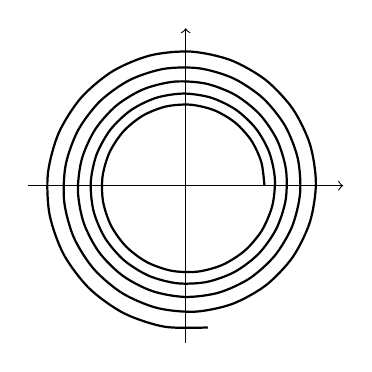
\begin{tikzpicture}
        \draw[->] (-2,0) -- (2,0);
        \draw[->] (0,-2) -- (0,2);
        \draw[domain=0:30,smooth,samples=100,variable=\x,thick]  plot ({exp(\x/50)*cos(deg(\x))},{exp(\x/50)*sin(deg(\x))});
      \end{tikzpicture}}
    \choice{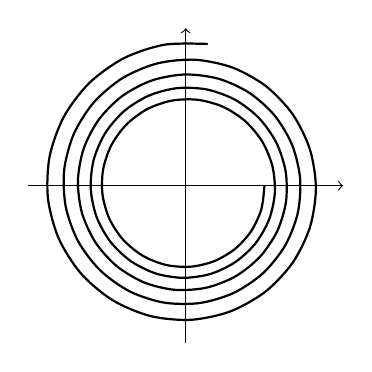
\begin{tikzpicture}
        \draw[->] (-2,0) -- (2,0);
        \draw[->] (0,-2) -- (0,2);
        \draw[domain=0:30,smooth,samples=100,variable=\x,thick]  plot ({exp(\x/50)*cos(-deg(\x))},{exp(\x/50)*sin(-deg(\x))});
      \end{tikzpicture}}    
    \choice{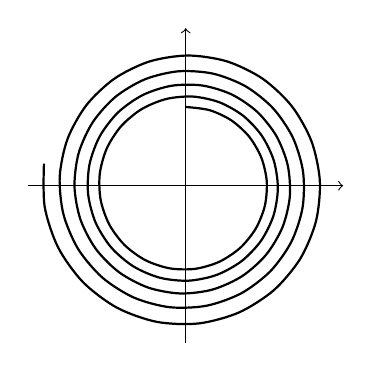
\begin{tikzpicture}
        \draw[->] (-2,0) -- (2,0);
        \draw[->] (0,-2) -- (0,2);
        \draw[domain=0:30,smooth,samples=100,variable=\x,thick]  plot ({exp(\x/50)*sin(deg(\x))},{exp(\x/50)*cos(deg(\x))});
      \end{tikzpicture}}    
    \choice{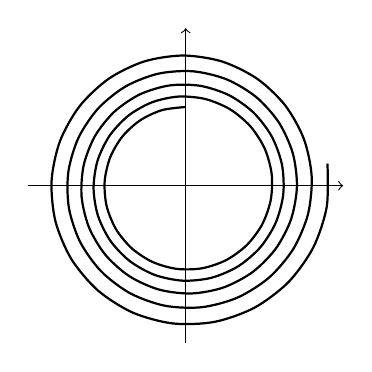
\begin{tikzpicture}
        \draw[->] (-2,0) -- (2,0);
        \draw[->] (0,-2) -- (0,2);
        \draw[domain=0:30,smooth,samples=100,variable=\x,thick]  plot ({exp(\x/50)*sin(-deg(\x))},{exp(\x/50)*cos(-deg(\x))});
      \end{tikzpicture}}    
  \end{multipleChoice}

\end{exercise}

\end{document}
